\documentclass[xelatex,aspectratio=169]{beamer}

\hfuzz=10pt
\vfuzz=10pt

% Theme
\usetheme{htw}
\setbeamertemplate{navigation symbols}{}
\setbeamertemplate{theorems}[numbered]
\setbeamercovered{transparent}

%\logo{
\includegraphics[height=0.5cm]{HTWD_color.png}}

% Packages
\usepackage{polyglossia}
\setmainlanguage{german}
\setotherlanguage{english}

\usepackage[bigfiles]{pdfbase}
\ExplSyntaxOn
\NewDocumentCommand\embedvideo{smm}{
\group_begin:
\leavevmode
\tl_if_exist:cTF{file_\file_mdfive_hash:n{#3}}{
  \tl_set_eq:Nc\video{file_\file_mdfive_hash:n{#3}}
}{
  \IfFileExists{#3}{}{\GenericError{}{File~`#3'~not~found}{}{}}
  \pbs_pdfobj:nnn{}{fstream}{{}{#3}}
  \pbs_pdfobj:nnn{}{dict}{
    /Type/Filespec/F~(#3)/UF~(#3)
    /EF~<</F~\pbs_pdflastobj:>>
  }
  \tl_set:Nx\video{\pbs_pdflastobj:}
  \tl_gset_eq:cN{file_\file_mdfive_hash:n{#3}}\video
}
%
\pbs_pdfobj:nnn{}{dict}{
  /Type/RichMediaInstance/Subtype/Video
  /Asset~\video
  /Params~<</FlashVars (
  source=#3&
  skin=SkinOverAllNoFullNoCaption.swf&
  skinAutoHide=true&
  skinBackgroundColor=0x5F5F5F&
  skinBackgroundAlpha=0.75
  )>>
}
%
\pbs_pdfobj:nnn{}{dict}{
/Type/RichMediaConfiguration/Subtype/Video
/Instances~[\pbs_pdflastobj:]
}
%
\pbs_pdfobj:nnn{}{dict}{
/Type/RichMediaContent
/Assets~<<
/Names~[(#3)~\video]
>>
/Configurations~[\pbs_pdflastobj:]
}
\tl_set:Nx\rmcontent{\pbs_pdflastobj:}
%
\pbs_pdfobj:nnn{}{dict}{
  /Activation~<<
  /Condition/\IfBooleanTF{#1}{PV}{XA}
  /Presentation~<</Style/Embedded>>
  >>
  /Deactivation~<</Condition/PI>>
}
%
\hbox_set:Nn\l_tmpa_box{#2}
\tl_set:Nx\l_box_wd_tl{\dim_use:N\box_wd:N\l_tmpa_box}
\tl_set:Nx\l_box_ht_tl{\dim_use:N\box_ht:N\l_tmpa_box}
\tl_set:Nx\l_box_dp_tl{\dim_use:N\box_dp:N\l_tmpa_box}
\pbs_pdfxform:nnnnn{1}{1}{}{}{\l_tmpa_box}
%
\pbs_pdfannot:nnnn{\l_box_wd_tl}{\l_box_ht_tl}{\l_box_dp_tl}{
  /Subtype/RichMedia
  /BS~<</W~0/S/S>>
  /Contents~(embedded~video~file:#3)
  /NM~(rma:#3)
  /AP~<</N~\pbs_pdflastxform:>>
  /RichMediaSettings~\pbs_pdflastobj:
  /RichMediaContent~\rmcontent
}
\phantom{#2}
\group_end:
}
\ExplSyntaxOff


\usepackage{graphicx}
\usepackage[export]{adjustbox}
\usepackage{animate}
%\usepackage[dvipdfmx]{movie15_dvipdfmx}
\usepackage{media9}
\usepackage{tabularx}
\usepackage{colortbl}
\usepackage{booktabs}
\usepackage{makecell}
\usepackage{ltablex}
\usepackage{array}
\usepackage{multirow}
\usepackage{amsmath}
\usepackage{amsthm}
%\renewcommand{\arraystretch}{1.5}
\newcolumntype{L}[1]{>{\raggedright\let\newline\\\arraybackslash\hspace{0pt}}p{#1}}
\newcolumntype{C}[1]{>{\centering\let\newline\\\arraybackslash\hspace{0pt}}p{#1}}
\newcolumntype{R}[1]{>{\raggedleft\let\newline\\\arraybackslash\hspace{0pt}}p{#1}}
%\renewcommand\thesatz{\arabic{section}.\arabic{theorem}}
\makeatletter
\@addtoreset{theorem}{lecture}
\makeatother

\newtheorem{satz}{Satz}[section]
\newtheorem{lem}{Lemma}[section]
\newtheorem{beh}{Behauptung}[section]
\newtheorem{define}{Definition}[section]
\numberwithin{equation}{section}
\usepackage{ragged2e}
\usepackage{etoolbox}

\usepackage{color}
\usepackage{colortbl}
\definecolor{hellgrau}{rgb}{0.85,0.85,0.85}
\definecolor{hellrot}{rgb}{1,0.7,0.7}

\usepackage{tikz}
\usetikzlibrary{shapes,arrows.meta,calc,arrows,positioning,patterns,tikzmark}
%\usepackage{tikz-uml}
\usepackage{pgfplots}  % for elliptic curves (part 8)
\pgfplotsset{compat=1.18}
\usepackage{pgffor}
\usepackage{pgfmath-xfp}
\tikzset{>=latex}
\tikzset{
  invisible/.style={opacity=0},
  visible on/.style={alt={#1{}{invisible}}},
  alt/.code args={<#1>#2#3}{%
      \alt<#1>{\pgfkeysalso{#2}}{\pgfkeysalso{#3}} % \pgfkeysalso doesn't change the path
    },
}

\usepackage{paralist}

\usepackage{url}
\def\UrlBreaks{\do\/\do-}
\PassOptionsToPackage{hyphens}{url}\usepackage{hyperref}

\usepackage[normalem]{ulem} % gestrichelte Unterstreichung (\dashuline{})
\usepackage{cancel}

\makeatletter
\renewcommand{\itemize}[1][]{%
  \beamer@ifempty{#1}{}{\def\beamer@defaultospec{#1}}%
  \ifnum \@itemdepth >2\relax\@toodeep\else
    \advance\@itemdepth\@ne
    \beamer@computepref\@itemdepth% sets \beameritemnestingprefix
    \usebeamerfont{itemize/enumerate \beameritemnestingprefix body}%
    \usebeamercolor[fg]{itemize/enumerate \beameritemnestingprefix body}%
    \usebeamertemplate{itemize/enumerate \beameritemnestingprefix body begin}%
    \list
    {\usebeamertemplate{itemize \beameritemnestingprefix item}}
    {\def\makelabel##1{%
        {%
            \hss\llap{{%
                  \usebeamerfont*{itemize \beameritemnestingprefix item}%
                  \usebeamercolor[fg]{itemize \beameritemnestingprefix item}##1}}%
          }%
      }%
    }
  \fi%
  \beamer@cramped%
  \justifying% NEW
  %\raggedright% ORIGINAL
  \beamer@firstlineitemizeunskip%
}
\makeatother

\apptocmd{\frame}{}{\justifying}{}

\renewcommand\theadfont{\bfseries\sffamily}
\usepackage{ragged2e}
\usepackage{newpxtext}

\setsansfont{texgyreheros}[
  Scale=MatchLowercase,
  UprightFont=*-regular,
  BoldFont=*-bold,
  ItalicFont=*-italic,
  BoldItalicFont=*-bolditalic,
]

% Title
\usepackage[usetransparent=false]{svg}
% Import references
\usepackage[backend=biber,style=numeric,sorting=none]{biblatex}
\addbibresource{references.bib}

%\AtBeginSection[]{
%  \begin{frame}
%    \vfill
%    \centering
%    \begin{beamercolorbox}[sep=8pt,center,shadow=true,rounded=true]{title}
%      \usebeamerfont{title}\thesection.~\secname\par%
%    \end{beamercolorbox}
%    \vfill
%  \end{frame}
%}

\makeatletter
\newenvironment{noheadline}{
  \setbeamertemplate{headline}{}
  \addtobeamertemplate{frametitle}{\vspace*{-0.9\baselineskip}}{}
}{}
\makeatother


\usepackage{xcolor}
\usepackage{algorithm}
\usepackage[linesnumbered,ruled,lined,commentsnumbered,algo2e,ngerman,ngermankw]{algorithm2e}
\usepackage{algorithmic}
\usepackage{caption}
\usepackage[newfloat]{minted}
\captionsetup[listing]{position=top}
\definecolor{mintedbg}{HTML}{282828}
\setminted{
  breaklines=true,
  bgcolor=mintedbg,
  style=monokai,
  formatcom=\color{white}
}
\usepackage{etoolbox}
\makeatletter
% replace \medskip before and after the box with nothing, i.e., remove it
\patchcmd{\minted@colorbg}{\medskip}{}{}{}
\patchcmd{\endminted@colorbg}{\medskip}{}{}{}
\makeatother

\renewcommand{\theFancyVerbLine}{\textcolor{black}{\arabic{FancyVerbLine}}}

\usepackage{pifont}
\newcommand{\cmark}{\ding{51}}%
\newcommand{\xmark}{\ding{55}}%

\newenvironment{changemargin}[2]{%
  \begin{list}{}{%
      \setlength{\topsep}{0pt}%
      \setlength{\leftmargin}{#1}%
      \setlength{\rightmargin}{#2}%
      \setlength{\listparindent}{\parindent}%
      \setlength{\itemindent}{\parindent}%
      \setlength{\parsep}{\parskip}%
    }%
    \item[]}{\end{list}}


\usepackage{csquotes}

% Title
\title{Simulation}
\author{Prof. Dr. Lukas Iffländer}
\institute{HTW Dresden}
\date{}
\usepackage{svg}

% Begin document
\begin{document}

% Title slide
\begin{frame}
    \titlepage
\end{frame}

\begin{frame}{Was ist Simulation?}
    \begin{block}{Definition (Wikipedia)}
        Die Simulation ist eine Vorgehensweise zur Analyse von Systemen, die für die theoretische oder formelmäßige Behandlung zu komplex sind. Dies ist überwiegend bei dynamischem Systemverhalten gegeben. Bei der Simulation werden Experimente an einem Modell durchgeführt, um Erkenntnisse über das reale System zu gewinnen.
    \end{block}
    \begin{block}{Definition (VDI)}
        Simulation ist das Nachbilden eines dynamischen Prozesses in einem System mit Hilfe eines experimentierfähigen Modells, um zu Erkenntnissen zu gelangen, die auf die Wirklichkeit übertragbar sind.
    \end{block}

\end{frame}

\begin{frame}{Arten von Simulation}
    \begin{block}{Nach Werteabbildung}
        \begin{itemize}
            \item Diskrete Simulation (endliche Anzahl von Zuständen)
            \item \textbf{Kontinuierliche Simulation} (Wertebereich unendlich)
        \end{itemize}
    \end{block}
    \begin{block}{Dynamisch vs. statisch}
        \begin{itemize}
            \item Statische Simulation (keine zeitliche Entwicklung)
            \item \textbf{Dynamische Simulation} (zeitliche Entwicklung)
        \end{itemize}
    \end{block}
    \begin{block}{Stochastisch vs. deterministisch}
        \begin{itemize}
            \item Stochastische Simulation (Zufallsvariablen, Wahrscheinlichkeiten)
            \item \textbf{Deterministische Simulation} (keine Zufallsvariablen)
        \end{itemize}
    \end{block}

\end{frame}

\begin{frame}{Explizites Euler-Verfahren}
    \begin{block}{Idee}
        Schrittweise Berechnung der Funktionswerte $y(t)$ für $t = t_{0 \cdot dt}, t_{1 \cdot dt}, \ldots, t_{n \cdot dt}$ mit Schrittweite $dt$.
    \end{block}

    \begin{block}{Verfahren}
        \begin{itemize}
            \item Kenntnis des Anfangswertes $y(t_0) = y_0$ und der Ableitung\footnote{erste Ableitung kann vorgegeben werden oder aus $y(t)$ und $t$ berechnet werden} $y'(t) = f(t, y)$.
            \item Approximation des Funktionswertes mit $y(t + dt) = y(t) + f(t, y) \cdot dt$.
        \end{itemize}
    \end{block}

    \begin{block}{Ergebnis}
        Kontinuierliches, dynamisches und deterministisches Simulationsverfahren.

    \end{block}
\end{frame}


\begin{frame}{Explizites Euler-Verfahren}{Wachstumsprozess}
    \begin{columns}[onlytextwidth]
        \begin{column}{0.5\textwidth}
            \inputminted[firstline=7, lastline=17]{python}{src/sim_growth.py}
        \end{column}
        \begin{column}{0.5\textwidth}
            \[
                \begin{aligned}
                    y(0)   & = 2                                      \\
                    y(1)   & = y(0) + f(0, y(0)) \cdot dt             \\
                           & = 2 + 0.5 \cdot 2 \ cdot 1 = 3           \\
                    y(2)   & = y(1) + f(1, y(1)) \cdot dt             \\
                           & = 3 + 0.5 \cdot 3 \cdot 1 = 4.5          \\
                    y(3)   & = y(2) + f(2, y(2)) \cdot dt             \\
                           & = 4.5 + 0.5 \cdot 4.5 \cdot 1 = 6.75     \\
                    y(4)   & = y(3) + f(3, y(3)) \cdot dt             \\
                           & = 6.75 + 0.5 \cdot 6.75 \cdot 1 = 10.125 \\
                    \cdots & \qquad\cdots                             \\
                \end{aligned}
            \]
        \end{column}
    \end{columns}
\end{frame}

\begin{frame}{Explizites Euler-Verfahren}{Fahrt mit wechselnder Geschwindigkeit}
    \begin{block}{Aufgabe}
        Fahrt mit zurückgelegter Strecke $s(t)$, Geschwindigkeit $v(t)$ ist vorgegeben und $v(t) = s'(t)$.
        \begin{columns}[onlytextwidth]
            \begin{column}{0.5\textwidth}
                \[
                    \begin{aligned}
                        s(0)    & = 0                    \\
                        dt      & = 0.1                  \\
                        s'(t)   & = v(t)                 \\
                        s(t+dt) & = s(t) + v(t) \cdot dt
                    \end{aligned}
                \]
            \end{column}
            \begin{column}{0.5\textwidth}
                \[
                    v(t) = \begin{cases}
                        0                                                  & t \leq 2        \\
                        (t-2) \cdot \frac{\mathrm{v_{max}}}{2}             & 2 \leq t < 4    \\
                        v_{max}                                            & 4 \leq t \leq 7 \\
                        v_{max} - (t - 7) \cdot \frac{\mathrm{v_{max}}}{3} & t \geq 7
                    \end{cases}
                \]
            \end{column}
        \end{columns}
    \end{block}

    \begin{block}{Berechnung}
        \[
            \begin{aligned}
                s(0)   & = 0                    \\
                s(0.1) & = s(0) + v(0) \cdot dt \\
                \cdots & \qquad\cdots           \\
            \end{aligned}
        \]
    \end{block}
\end{frame}
\begin{frame}{Explizites Euler-Verfahren}{Fahrt mit wechselnder Geschwindigkeit}
    \begin{columns}
        \begin{column}{0.5\textwidth}
            \small
            \inputminted[firstline=8, lastline=17]{python}{src/sim_drive.py}
        \end{column}
        \begin{column}{0.5\textwidth}
            \small
            \inputminted[firstline=20, lastline=30]{python}{src/sim_drive.py}
        \end{column}
    \end{columns}
\end{frame}

\begin{frame}{Explizites Euler-Verfahren}{Fahrt mit wechselnder Geschwindigkeit}
    \inputminted[firstline=33, lastline=42]{python}{src/sim_drive.py}
\end{frame}

\begin{frame}{Explizites Euler-Verfahren}{Fahrt mit wechselnder Geschwindigkeit}
    \begin{columns}[T]
        \begin{column}{0.5\textwidth}
            \inputminted[lastline=12]{python3}{src/sim_drive_result.txt}
        \end{column}
        \begin{column}{0.5\textwidth}
            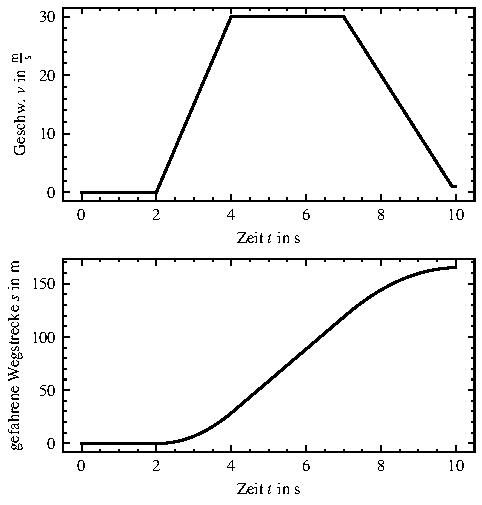
\includegraphics[height=.8\textheight]{fig/sim_drive_plot.pdf}
        \end{column}
    \end{columns}
\end{frame}

\begin{frame}{Einschub}{SciencePlots}
    \begin{block}{Was ist SciencePlots?}
        \begin{itemize}
            \item Python-Paket für ansprechende Matplotlib-Plots
            \item Einfach zu verwenden, nur ein Import nötig
            \item Viele vordefinierte Stile
        \end{itemize}
    \end{block}

    \begin{block}{Installation}
        \begin{itemize}
            \item Installation mit pip: \texttt{pip install SciencePlots}
            \item Import in Python: \texttt{import SciencePlots}
            \item Aktivierung mit \texttt{plt.style.use(["science", "ieee"])}
            \item Stile können angepasst und kombiniert werden
            \item Wenn Schwarz-Weiß-Druck relevant ist, empfiehlt sich der Stil \texttt{"ieee"}.
        \end{itemize}
    \end{block}

\end{frame}

\begin{frame}{Explizites Euler-Verfahren}{Logistisches Wachstum}
    Wachstumsprozess mit Sättigung, z.B. Populationswachstum.
    \begin{block}{Modell}
        \begin{columns}[onlytextwidth]
            \begin{column}{0.5\textwidth}
                \[
                    \begin{aligned}
                        dt        & = 1                             \\
                        y(0)      & = 2                             \\
                        y'(t)     & = f(K, N, y(t))                 \\
                        y(t + dt) & = y(t) + f(K, N, y(t)) \cdot dt
                    \end{aligned}
                \]
            \end{column}
            \begin{column}{0.5\textwidth}
                \[
                    \begin{aligned}
                        y'(t) & = K \cdot y(t) \cdot \left(1 - \frac{y(t)}{N}\right) \\
                        K     & \qquad\text{Wachstumsrate}                           \\
                        N     & \qquad\text{Wachstumsgrenze}                         \\
                    \end{aligned}
                \]
            \end{column}
        \end{columns}
    \end{block}
\end{frame}

\begin{frame}{Explizites Euler-Verfahren}{Logistisches Wachstum}
    \begin{columns}
        \begin{column}{0.5\textwidth}
            \inputminted[firstline=13,lastline=25]{python}{src/sim_growth_log.py}
        \end{column}
        \begin{column}{0.5\textwidth}
            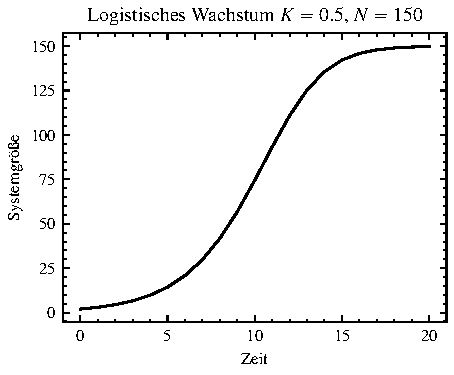
\includegraphics[width=\textwidth]{fig/sim_growth_log.pdf}
        \end{column}
    \end{columns}
\end{frame}

\begin{frame}{Explizites Euler-Verfahren}{Mehr Ableitungen}
    Simulation einer Fahrt mit gegebenen Beschleunigungswerten.
    \begin{block}{Modell}
        Gegeben:
        \begin{itemize}
            \item Anfangsgeschwindigkeit $v_0 = 0$
            \item Anfangsposition $s_0 = 0$
            \item Beschleunigung $a(t)$ für $t$-Intervalle
        \end{itemize}
        Zusammenhänge:
        \begin{itemize}
            \item Geschwindigkeit: Erste Ableitung des Weges $s$ nach der Zeit $t$: $v(t) = s'(t)$
            \item Beschleunigung: Erste Ableitung der Geschwindigkeit $v$ nach der Zeit $t$: $a(t) = v'(t)$
            \item Weg: Zweite Ableitung der Position $s$ nach der Zeit $t$: $a(t) = s''(t)$
        \end{itemize}
    \end{block}
\end{frame}

\begin{frame}{Explizites Euler-Verfahren}{Mehr Ableitungen}
    Umwandlung der DGL zweiter Ordnung $a(t) = s''(t)$ in zwei DGL erster Ordnung:
    \begin{itemize}
        \item $v(t) = s'(t)$
        \item $a(t) = v'(t)$
    \end{itemize}
    Für Simulationsschritt gilt dann:
    \begin{itemize}
        \item $s(t + dt) = s(t) + v(t) \cdot dt$
        \item $v(t + dt) = v(t) + a(t) \cdot dt$
    \end{itemize}
\end{frame}
\begin{frame}{Explizites Euler-Verfahren}{Mehr Ableitungen}
    \begin{columns}
        \begin{column}{0.5\textwidth}
            \inputminted[firstline=10, lastline=22]{python}{src/sim_growth_2nd.py}
        \end{column}
        \begin{column}{0.5\textwidth}
            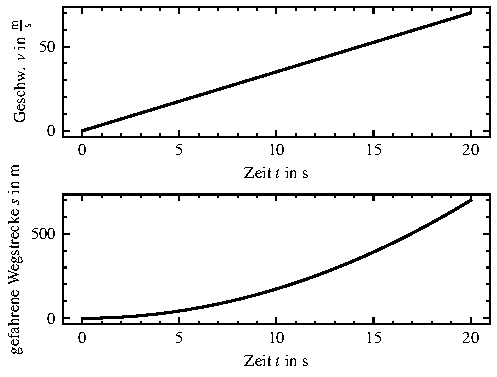
\includegraphics[width=\textwidth]{fig/sim_growth_2nd.pdf}
        \end{column}
    \end{columns}
\end{frame}

\begin{frame}{Explizites Euler-Verfahren}{Pendelsimulation}
    \begin{block}{Modell}
        Gegeben:
        \begin{itemize}
            \item DGL 2. Ordnung: $a''(t) = -\frac{g}{l} \cdot \sin(\alpha(t))$
            \item Anfangswerte für Winkel $\alpha(0) = \alpha_0 = \frac{\pi}{4}$ und Winkelgeschwindigkeit $\omega(0) = \omega_0 = 0$
            \item Parameter: $g$ (Erdbeschleunigung), $l$ (Länge des Pendels)
        \end{itemize}
    \end{block}
    \begin{block}{Berechnung}
        Wieder Zerlegung in zwei DGL erster Ordnung:
        \begin{itemize}
            \item $\alpha'(t) = \omega(t)$
            \item $\omega'(t) = -\frac{g}{l} \cdot \sin(\alpha(t))$
        \end{itemize}
        Für Simulationsschritt gilt dann:
        \begin{itemize}
            \item $\alpha(t + dt) = \alpha(t) + \omega(t) \cdot dt$
            \item $\omega(t + dt) = \omega(t) - \frac{g}{l} \cdot \sin(\alpha(t)) \cdot dt$
        \end{itemize}
    \end{block}
\end{frame}

\begin{frame}{Explizites Euler-Verfahren}{Pendelsimulation}
    \begin{columns}
        \begin{column}{0.5\textwidth}
            \inputminted[firstline=10, lastline=21]{python}{src/sim_pendel.py}
        \end{column}
        \begin{column}{0.5\textwidth}
            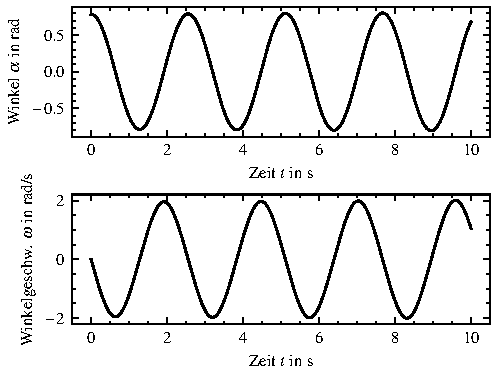
\includegraphics[width=\textwidth]{fig/sim_pendel.pdf}
        \end{column}
    \end{columns}
\end{frame}

\begin{frame}{Explizites Euler-Verfahren}{Abhängigkeiten}
    \begin{columns}
        \begin{column}{0.5\textwidth}
            \begin{block}{Model}
                Wildschweinbestand und Wolfsbestand, vorerst ohne Beeinflussung
                \begin{itemize}
                    \item Wildschweine $b$
                          \begin{itemize}
                              \item Anfangsbestand $b(0) = 2000$
                              \item Wachstumsrate $K_b = 0.6$
                              \item Wachstumsgrenze $N_b = 4000$
                          \end{itemize}
                    \item Wölfe $w$
                          \begin{itemize}
                              \item Anfangsbestand $w(0) = 20$
                              \item Wachstumsrate $K_w = 0.1$
                              \item Wachstumsgrenze $N_w = 1000$
                          \end{itemize}
                \end{itemize}
            \end{block}
        \end{column}
        \begin{column}{0.5\textwidth}
            \smaller
            \inputminted[firstline=7, lastline=21]{python}{src/sim_dependency_a.py}
        \end{column}
    \end{columns}
\end{frame}

\begin{frame}{Explizites Euler-Verfahren}{Abhängigkeiten}
    \centering
    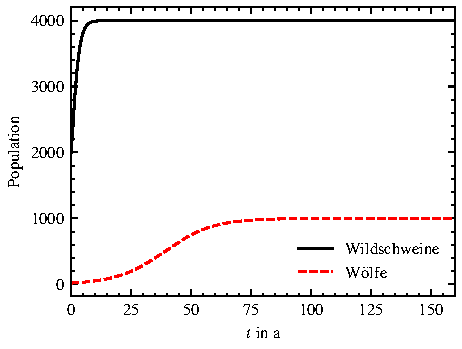
\includegraphics[height=.8\textheight]{fig/sim_dependency_a.pdf}
\end{frame}

\begin{frame}{Explizites Euler-Verfahren}{Abhängigkeiten}
    \begin{block}{Model}
        Ein Wolf frisst jedes Jahr eine bestimmte Anzahl Wildschweine
    \end{block}
    \inputminted[firstline=19, lastline=23]{python}{src/sim_dependency_b.py}
\end{frame}

\begin{frame}{Explizites Euler-Verfahren}{Abhängigkeiten}
    \centering
    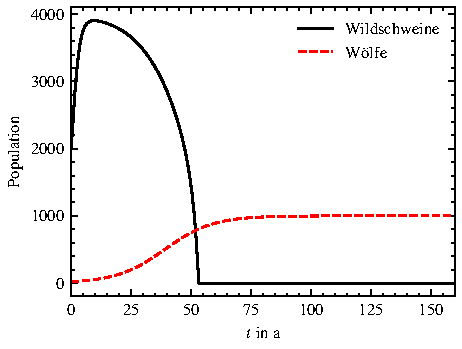
\includegraphics[height=.8\textheight]{fig/sim_dependency_b.pdf}
\end{frame}

\begin{frame}{Explizites Euler-Verfahren}{Abhängigkeiten}
    \begin{block}{Model}
        Alle 10 Jahre wird die Anzahl der Wölfe um 40\% reduziert.
    \end{block}
    \inputminted[firstline=19, lastline=23]{python}{src/sim_dependency_c.py}
\end{frame}

\begin{frame}{Explizites Euler-Verfahren}{Abhängigkeiten}
    \centering
    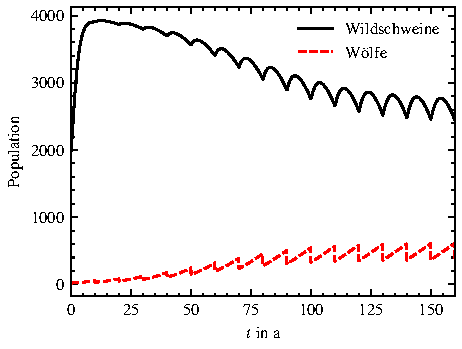
\includegraphics[height=.8\textheight]{fig/sim_dependency_c.pdf}
\end{frame}

\end{document}
